\section{Durchführung}

    	In dem Aufbau wird die Geschwindigkeit von kleinen Glaskugeln in einer Flüssigkeit gemessen.
        Diese fließt durch eine Röhre mit der Flussgeschwindigkeit $v_{\symup{F}}$. Dafür ein
        Ultraschallgerät, welches sowohl Wellen aussendet, als auch empfängt, an ein Prisma mit
        einer Schicht aus Gel gehalten. Zwischen das Prisma und den Schlauch kommt eine weitere
        Gelschicht, um den Einfluss von den Störungen durch Luft zu minimieren. 
        Das Ultraschallgerät misst hierbei die Frequenzverschiebung, die von den Glaskugeln
        verursacht wird und gibt deren Mittelwert auf dem Bildschirm aus. \\

        \begin{figure}[H]
            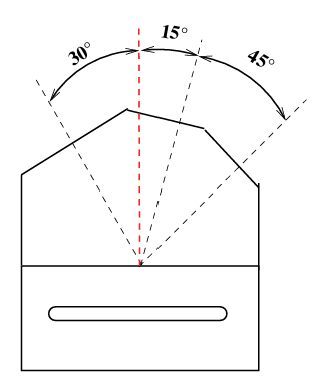
\includegraphics{Bilder/winkel.png}
            \label{fig:winkel}       
        \end{figure}
        \noindent Die Prismen haben hierbei Flächen, die wie in Abbildung \ref{fig:winkel} geneigt sind.
        An diesen Flächen wird das Ultraschallgerät drangehalten. Für jeden Winkel wird dann die mittlere
        Frequenzverschiebung gemessen für Flussgeschwindigkeiten zwischen $v_{\symup{F}}=\qty{3}{\meter\per\second}\text{ bis }
        \qty{7}{\meter\per\second}$ in Schritten von $\qty{1}{\meter\per\second}$. Dies wird zweimal für die
        Rohrdicken $d_1=\qty{7}{\milli\meter}$ und $d_2=\qty{16}{\milli\meter}$ durchgeführt.\\
        \noindent Danach wird bei der Frequenzmessung die Messtiefe für spezifische Flussgeschwindigkeiten gemessen.
        Für die Messung wird der Winkel aus Abbildung \ref{fig:winkel} auf 15° festgehalten. Dabei wird die Messung
        bei den Schlauchdicken $d_1=\qty{7}{\milli\meter}$ und $d_3=\qty{10}{\milli\meter}$ durchgeführt mit 
        Flussgeschwindigkeiten von jeweils $v_{\symup{F}1}=\qty{3}{\liter\per\minute}$ und $v_{\symup{F}2}=\qty{6}{\liter\per\minute}$.
        
\label{sec:Durchführung}
